
\section*{Key Research Directions}

%Identify capability gaps and define research objectives that integrate autonomy and humans (as command, analysts, operators, and soldiers) that are:
%Model-based, probabilistic, and verifiable (correct by construction)
%Scalable: self-organizing networks of heterogeneous actors that perform navigation, sensing, communication, and computation
%Agile: can be rapidly validated and deployed for specific exploitation missions
%

Given the motivation from the DSB and other DoD studies, and the background in these five areas, our goal was to identify capability gaps and key research objectives that integrate autonomy and humans (as command, analysts, operators, and soldiers) that are:\vspace*{-0.1 in}
\begin{itemize}
\item Model-based, probabilistic, and verifiable (correct by construction)\vspace*{-0.1 in}
\item Scalable: self-organizing networks of heterogeneous actors that perform navigation, sensing, communication, and computation\vspace*{-0.1 in}
\item Agile: can be rapidly validated and deployed for specific exploitation missions\vspace*{-0.1 in}
\end{itemize}

Four research directions are described below that will enable these goals. 

\subsection*{Probabilistic Models of Human Capabilities in Correct by Construction Frameworks}

A key research direction is to leverage probabilistic models of human capabilities, and integrate these models into formal frameworks that enable the generation of correct by construction controllers for autonomous systems. Importantly, not all human capabilities have to be modeled; only {\it some} capabilities. And, these models can be probabilistic because the current state of the art in formal methods includes formal tools that consider probability. 

These models can be derived from underlying knowledge of human capabilities, but will mostly be derived from data collected from human tests. Models could be general (a group of humans), or custom (a specific person). A key challenge is minimizing the data collection required to develop such models.  As models of human capabilities mature, they can be integrated into the same framework, and new controllers will be automatically generated that are richer in their ability to work together with humans. 

If a framework exists whereby probabilistic models of human capabilities are integrated into a verifiable framework, then we could:
\vspace*{-0.1 in}
\begin{itemize}
\item Automatically verify (and auto-generate) correct by construction controllers for autonomy. These controllers would be designed with the {\it integrated} human+autonomous system in mind because the specifications are on the task itself, and the models include both the humans and autonomy.  \vspace*{-0.1 in}
\item Generate autonomy software that is `matched' to human capabilities. Given that a different probabilistic model of human capabilities could be developed for different people, it is envisioned that the associated controllers that are automatically generated will consider each person individually. \vspace*{-0.1 in}
\item Speed validation. In any V\&V framework, any improvement in verification (such as increasing speed with automatic verification of formal methods), will in turn speed the end validation process.  \vspace*{-0.1 in}
\end{itemize}

As an example, consider the case of a network of humans and autonomous robots working together on a task, such as surveillance of an area, rescue mission in a forest or building, or other. Figure~\ref{fig:collaboration} shows an abstraction of such a network, with $N$ autonomous vehicles. For this example, we will assume that the human analyzes data feeds for objects and false detections. During a prior testing, models of human capabilities of three particular operators showed that they each have important characteristics:\vspace*{-0.1 in}
\begin{itemize}
\item Operator A has faster eye-hand coordination\vspace*{-0.1 in}
\item Operator B has a photographic memory\vspace*{-0.1 in}
\item Operator C's performance drops rapidly with task load\vspace*{-0.1 in}
\end{itemize}

Given models of these capabilities, the concept of {\it `personalized autonomy'} can be realized whereby the correct-by-construction controller for the autonomous takes these abilities into account. Importantly, the controller is designed with {\it collaborative performance} for the task in mind, not separately. This capability would be useful not only for the original design effort, but also operational deployment with the concept of adaptive tasking~\cite{parasuraman2009adaptive}.

\begin{figure}[h] %  figure placement: here, top, bottom, or page
   \centering
   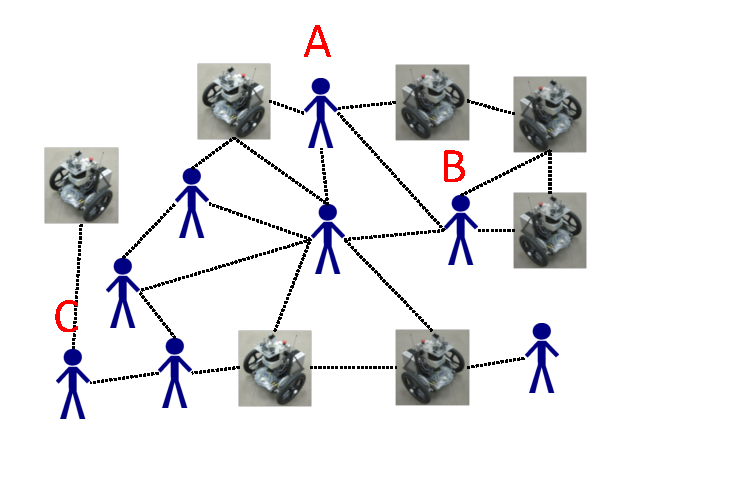
\includegraphics[height=1.5in]{collaboration.pdf} 
   \caption{A network of humans and autonomous systems working together on a task.}
   \label{fig:collaboration}
\end{figure}



\subsection*{Rapid Validation}

A key challenge in future systems is the speed and ability to validate systems prior to deployment. Future autonomy (adaptive, agile) are near infinite state systems, and traditional empirical validation (Test \& Evaluate, T\&E) will not scale~\cite{tech-horizons2011}. 

An example from the DARPA Urban Challenge (DUC) in 2007 crystallized these challenges~\cite{Campbell2010e,Miller2008}. The Cornell team developed an autonomous driving car for the competition. In the 12-18 months prior to the competition, the Cornell team tested and evaluated sub-components and the integrated system, with much of the final six months devoted to systems level testing and evaluation (i.e.\ validation). During the semi-finals of the DUC, Cornell's car, Skynet, could not navigate through a course with many cars parked in either side of the road; this was because the road was narrow, and Skynet is large (a Chevrolet Tahoe). The only way to navigate the course was enable Skynet to slightly cross over the double yellow line in the middle of the road - a capability that the Cornell team took great lengths to avoid. 

In order to make it into the DUC finals, the Cornell team had to make a small software change (a few lines of code) in order to enable Skynet to navigate closer to side cars and over the double yellow line. However, the Cornell team kept asking the same questions: {\it Will this change create other problems? Will this change invalidate the months of validation tests that the team had completed}. In the end, Skynet completed both the semi-finals and finals, completing the competition as one of six finishers. However, not without a lot of stress about not knowing the effects of such a small change. 

One `promise' of a verifiable, probabilistic, correct by construction framework is a shorter validation time. We envision that such tools will enable this improvement. Consider the case of a single operator and UAV, working together on a surveillance task (Figure~\ref{fig:uav-operator}). The specific task is to find and identify certain people in crowded spaces. The operator and UAV must work together on such a task, as the UAV must position itself appropriately (height, location); search and maintain camera field of view on important people; continue to fly why completing its sensing task. The human tasks the UAV to a general area, watches the video, and picks the object of interest that the UAV must track. Consider that the UAV, software, and operator interface were developed, and validation tests occurred over many months that demonstrated reliability to a high level of probability. 

Here is an important question: {\it After one year in operation, the DoD wants to add a new capability, that of automatic entity detection in the UAV software, and use this detection to re-task the UAV.}  Will the past T\&E validation be invalidated? i.e.\ not useful any more? Or can some be used? How much additional T\&E is required to deploy the system again? 

Further, acceptance should be based on the completed task (search, ID, track objects on the ground), and this task is dependent on {\it both} the human and UAV. Thus, if the UAV performs better at its tasks, but the human does not understand/trust the new software, the {\it integrated} human+UAV system could perform worse than it did previously. 

%Example:
%Sensory UAV
%Deployed after FULL test and evaluation (T\&E)
%After a year in operation, would like to add new capability:
%Automatic entity detection for re-tasking
%Past: Need T\&E again?
%Future: Auto-generation of correct by construction (verified) software

\begin{figure}[h] %  figure placement: here, top, bottom, or page
   \centering
   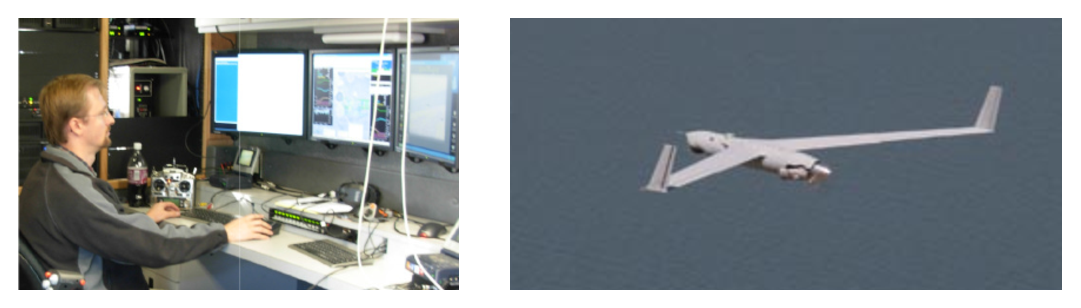
\includegraphics[height=1.5in]{uav-operator.pdf} 
   \caption{An operator tasking a UAV. }
   \label{fig:uav-operator}
\end{figure}

%MC try to Merge with the example. (one slide)
%Takeaway is for a general or Arthi
%Cite Dahm smally
%from SOA and correctness
%Yellow line / car example (?)

While the proposed framework may not solve all problems, it is conceivable that if the software for the UAV was auto-generated to create probabilistically correct by construction (verified) software, then it is conceivable that the addition of UAV capabilities (and perhaps some human tests/models) would enable a faster verification process. 



\subsection*{Multi-scale architectures for human autonomy}

\rb{TODO}

\subsection*{Human-Automation System Co-Design}

\ella{TODO}

